\documentclass[a4paper, 12pt]{article}
\usepackage[top=2cm, bottom=2cm, left=2.5cm, right=2.5cm]{geometry}
\usepackage[utf8]{inputenc}
\usepackage[brazilian]{babel}
\usepackage{indentfirst}
\usepackage{graphicx}
\usepackage{wrapfig}
\usepackage[pdftex]{hyperref}
\graphicspath{ {imagens/} }

\begin{document}
%
\begin{titlepage} %iniciando a "capa"
	\begin{center} %centralizar o texto abaixo
		{\large Unicamp}\\[0.2cm] %0,2cm é a distância entre o texto dessa linha e o texto da próxima
		{\large [Matéria]}\\[0.2cm] % o comando \\ "manda" o texto ir para próxima linha
		{\large [Professor]}\\[3.2cm]
		{\bf \huge TÍTULO}\\[0.2cm] 
		{\bf \large Subtítulo}\\[4.9cm]
		% o comando \bf deixa o texto entre chaves em negrito. O comando \huge deixa o texto enorme
	\end{center} %término do comando centralizar
	{\large Erik Yuji Goto}\\[10cm] % o comando \large deixa o texto grande
	\begin{center}
	
		{\large Campinas}\\[0.2cm]
		{\large 2020}
	\end{center}
\end{titlepage} %término da "capa"


\tableofcontents
\newpage

\section{Conceitos Iniciais}
	\subsection{Velocidade Instântanea}
		\begin{center}
			\Large			
			$
			\vec{v(t)} = \frac{d\vec{r}}{dt}[\frac{m}{s}]			
			$
		\end{center}
	\subsection{Aceleração Instântanea}
		\begin{center}
			\Large			
			$
			\vec{a(t)}_m = \frac{d\vec{v}}{dt} = \frac{d^2\vec{r}}{d^2t} [\frac{m^2}{s}]			
			$
		\end{center}
	
	\subsection{Velocidade Angular}
		\begin{center}
			\Large			
			$
			\omega = \frac{d\theta}{dt} [\frac{rad}{s}]	
			$\\
			$
			\vec{\omega} = \dot{\theta}\hat{k}
			$			
			
		\end{center}
		
	\subsection{Aceleração Angular}
		\begin{center}
			\Large			
			$
			\alpha = \frac{d\omega}{dt} = \frac{d^2\theta}{dt^2}[\frac{rad}{s^2}]	
			$\\
			$
			\vec{\alpha} = \ddot{\omega}\hat{k}
			$			
			
		\end{center}

\section{Movimento Retilíneo da Partícula}
	\begin{figure}[h]
		\center
		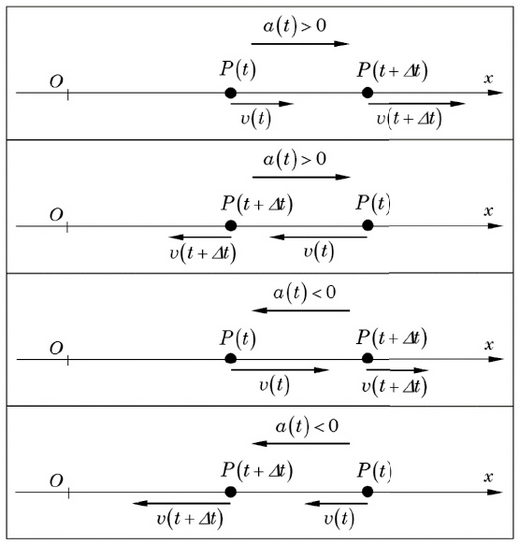
\includegraphics[scale=0.45]{imagens/mr.png} 
		\caption{Movimentos retilíneos}
	\end{figure}		
	
	\begin{enumerate}
		\item $v(t) = v_0 + at$
		\item $x(t) = x_0 + v_0t + \frac{1}{2}at^2$
		\item $v^2(x) = v_0^2+2a(x-x_0)$ - Torricelli
		\item $x(t) = x_0 + vt$
	\end{enumerate}

\section{Moviento Curvilíneo da Partícula}
	\subsection{Coordenadas Cartesianas}
		\begin{figure}[h]
			\center
			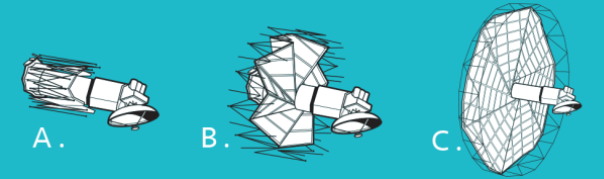
\includegraphics[scale=0.5]{imagens/c.png} 
			\caption{Cartesianas}
		\end{figure}	
		
		\begin{enumerate}
			\item $\vec{v}(t) = \dot{x}(t)\vec{i} + \dot{y}(t)\vec{j}$
			\item $\vec{a}(t) = \ddot{x}(t)\vec{i} + \ddot{y}(t)\vec{j}$
		\end{enumerate}
	\subsection{Coordenadas Normal-Tangencial}
		\begin{figure}[h]
			\center
			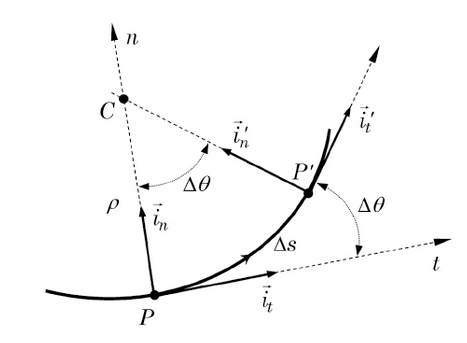
\includegraphics[scale=0.5]{imagens/t.png} 
			\caption{Normal-tangencial}
		\end{figure}		

		\begin{enumerate}
			\item $\vec{v}(t) = v(t) \hat{i}_t$
			\item $\vec{a}(t) = \frac{dv}{dt} \hat{i}_t + \frac{v^2}{\rho} \hat{i}_n$
		\end{enumerate}
	
	\subsection{Coordenadas Polares}
		\begin{figure}[h]
			\center
			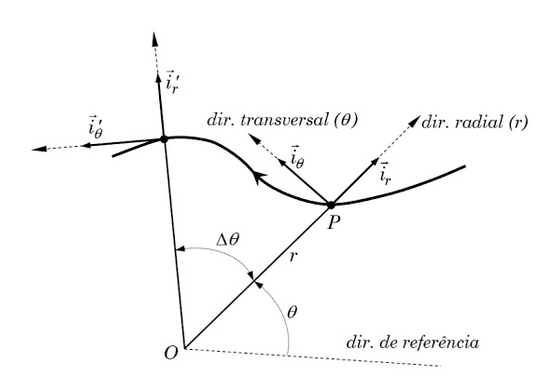
\includegraphics[scale=0.5]{imagens/pol.png} 
			\caption{Polares}
		\end{figure}	
		
		\begin{enumerate}
			\item $\vec{v}(t) = \dot{r}\vec{i}_r + r\dot{\theta} \vec{i}_{\theta}$
			\item $\vec{a}(t) = (\ddot{r} - r\dot{\theta}^2)\vec{i}_r + (r\ddot{\theta} + 2 \dot{r}\dot{\theta})\vec{i}_{\theta}$
		\end{enumerate}

\section{Movimento Circular}
	\begin{center}
		\Large
		$
		\vec{v} = (r\omega)\vec{i}_{\theta}		
		$\\
		$
		\vec{a} = (-r\omega^2)\vec{i}_r + (r\alpha)\vec{i_\theta}		
		$\\ \textit{ou}\\
		$
		\vec{v} = \vec{\omega} \times \vec{r}	
		$\\
		$
		\vec{\alpha} = \vec{\alpha} \times \vec{r} - \omega^2\vec{r}	
		$
	\end{center}

\section{Movimento Curvilíneo Espacial da Partícula}
	\subsection{Coordenadas Cartesianas}
		\begin{figure}[h]
			\center
			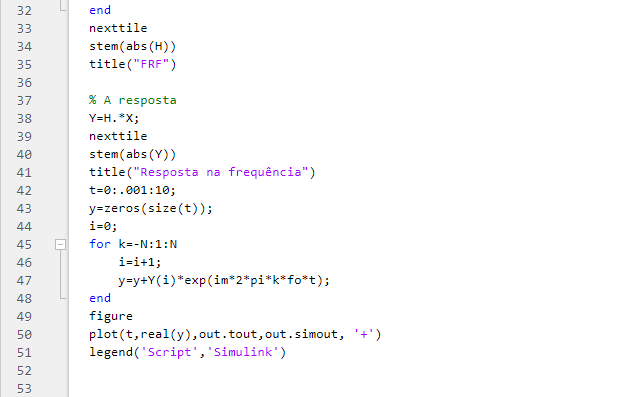
\includegraphics[scale=0.5]{imagens/cc.png} 
			\caption{Cartesianas}
		\end{figure}	
		\newpage
		\begin{figure}[h]
			\center
			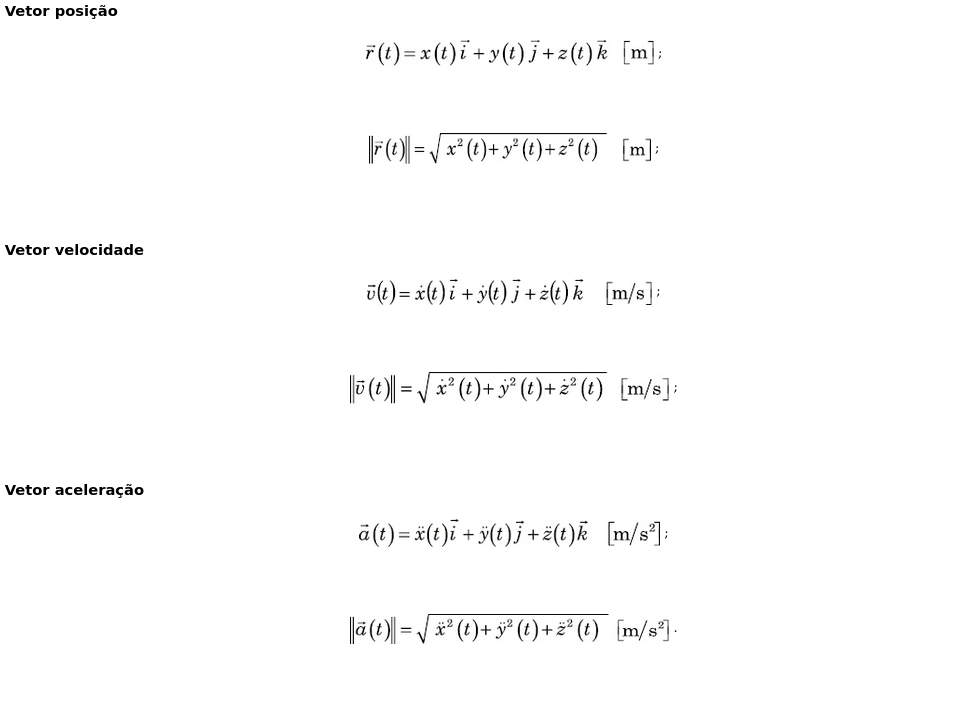
\includegraphics[scale=0.6]{imagens/ccc.png} 
			\caption{Cartesianas}
		\end{figure}

	\subsection{Coordenadas Cilíndricas}
		\begin{figure}[h]
			\center
			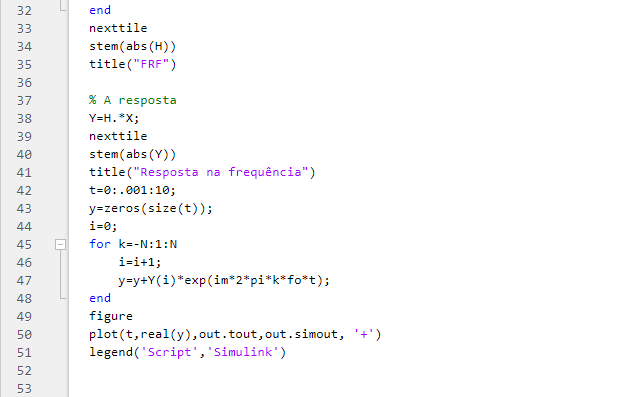
\includegraphics[scale=0.5]{imagens/cc.png} 
			\caption{Cilíndricas}
		\end{figure}	
		
		\begin{enumerate}
			\item $\vec{v} = \dot{r}\vec{i}_r + r\dot{\theta}\vec{i}_{\theta} + \dot{z}\vec{k}$
			\item $\vec{a} = (\ddot{r} - \dot{r}\dot{\theta}^2)\vec{i_r} + (r\ddot{\theta} + 2\dot{r}\dot{\theta})\vec{i_{\theta}} + \ddot{z}\vec{k}$
		\end{enumerate}
	\newpage
	\subsection{Coordenadas Esféricas}
		\begin{figure}[h]
			\center
			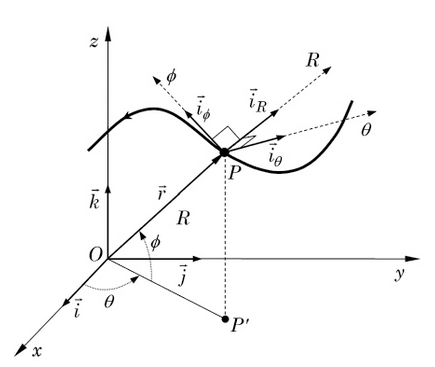
\includegraphics[scale=0.5]{imagens/e.png} 
			\caption{Esféricas}
		\end{figure}
	\begin{enumerate}
		\item $\vec{v} = \dot{R}\vec{i_R} + R\dot{\theta}cos\phi\vec{i_{\theta}} + R\dot{\phi}\vec{i}_{\phi}$
		\item 
	\end{enumerate}
		\begin{figure}[h]
			\center
			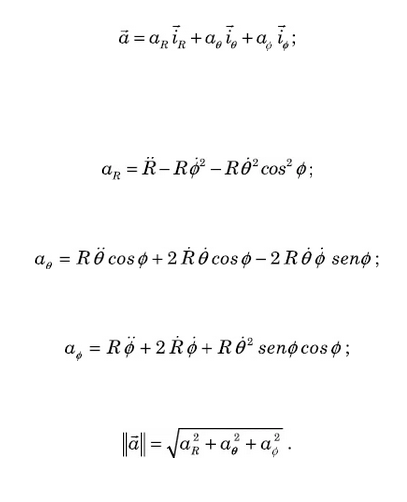
\includegraphics[scale=0.5]{imagens/ee.png} 
		\end{figure}	

\section{Transformações de Coordenadas}
\newpage

\section{Movimento Relativo}
	\subsection{Plano - Eixos de Referência em Translação}
	\begin{figure}[h]
		\center
		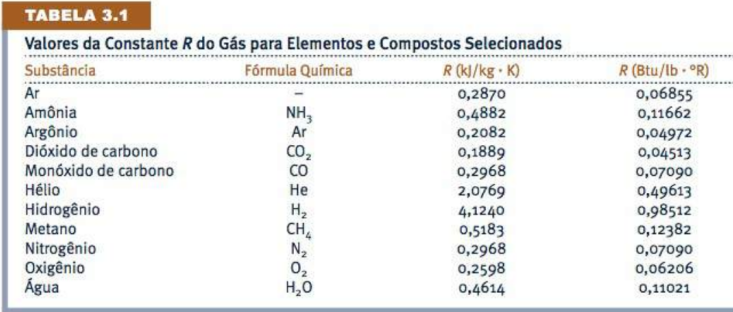
\includegraphics[scale=0.5]{imagens/r.png} 
		\caption{Cilíndricas}
	\end{figure}	

	\begin{enumerate}
		\item $\vec{r}_p = \vec{r}_A + \vec{r}_{P/A}$
		\item $\vec{v}_p = \vec{v}_A + \vec{v}_{P/A}$
		\item $\vec{a}_p = \vec{a}_A + \vec{a}_{P/A}$
	\end{enumerate}

	\subsection{Plano - Eixos de Referência em Rotação}
		\begin{figure}[h]
			\center
			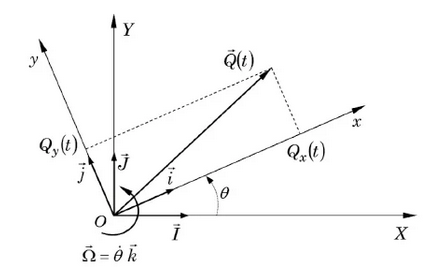
\includegraphics[scale=0.5]{imagens/rr.png} 
			\caption{Cilíndricas}
		\end{figure}	

		\begin{enumerate}
			\item $\vec{v}_p|_{OXY} = \vec{\dot{r}}_P|_{Oxy} + \vec{\Omega}\times\vec{r}_P$
			\item $\vec{a}_P|_{OXY} = \vec{\ddot{r}}_P|_{Oxy} + \vec{\dot{\Omega}}\times \vec{r}_p - \vec{\Omega}^2\vec{r}_P + 2\vec{\Omega}\times \vec{\dot{r}}_P|_{Oxy}$
		\end{enumerate}
		
	\newpage
	\subsection{Plano - Eixos de Referência em Movimento Geral}
		\begin{figure}[h]
			\center
			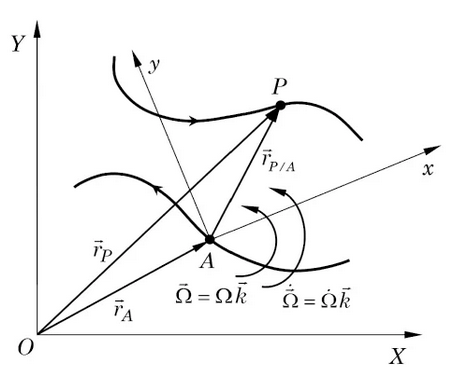
\includegraphics[scale=0.5]{imagens/ra.png} 
			\caption{Cilíndricas}
		\end{figure}	

		\begin{enumerate}
			\item $\vec{v}_P|_{OXY} = \vec{\dot{r}}_A|_{OXY} + \vec{\dot{r}}_{P/A}|_{Axy} + \vec{\Omega} \times \vec{r}_{P/A}$
			\item $\vec{a}_P|_{OXY} = \vec{\ddot{r}}_A|_{OXY} + \vec{\ddot{r}}_{P/A}|_{Axy} + \vec{\dot{\Omega}}\times \vec{r}_{P/A} - \vec{\Omega}^2\vec{r}_{P/A} + 2\vec{\Omega}\times \vec{\dot{r}}_{P/A}|_{Axy}$
		\end{enumerate}




















\end{document}
